%%
%% This is file `introduction.tex',
%%
The engineering standard for blast-resistant design is the Unified Facilities Criteria (UFC) 3-340-02 \cite{UFC3-340-02-2008}.  It is used extensively in the United States, United Kingdom, Australia, and Canada.   The primary blast-parameters used for protective design in the UFC are the:
\begin{itemize}
  \item incident-pressure,
  \item incident-impulse,
  \item reflected-pressure, and
  \item reflected-impulse.
\end{itemize}

The Kingery-Bulmash (KB) equations are used to estimate these blast-parameters in the UFC.  The equations are presented as a series of charts (free-air spherical and surface hemispherical) and are based on higher-order polynomials \cite{Kingery1984}.  Large scale testing of the explosive, trinitrotoluene (TNT), was used to develop the equations.  Because the equaitons are curve fits of test data, they are only valid over the scaled distances of the corresponding tests, $Z = 0.134 - 100$, where, 

$$Z=R/W^{1/3}$$
and $R$ is the distance from the center of the charge to the point of interest and $W$ is the charge weight (mass). 

There are some interesting local maxima in the KB equations that occur at small scaled distances.  In particular, the incident impulse and positive phase duration show local maxima , see Figure \ref{fig:KB_ip_ppd_ii}.  This is particularly evident with the incident impulse. is a function of peak pressure and time.  Therefore it is logical to assume that the maximum in the impulse is correlated to if not caused by the maxima in the positive phase duration.  Another interesting observation is that none of the other KB curves (there are a total of 8 for a given charge configuration ) show any local maxima including the reflected impulse and positive phase duration.  The local maximum results in an increase in the incident-impulse at scaled distances above $1.0\:\frac{ft}{\sqrt[3]{lb}}$.  On average the incident impulse is increased by $15$ times compared to a curve where no local maximum occurs, see Figure \ref{fig:KB_avg_inc}.  The increase in incident impulse results in a larger design load on any nearby structures. Unfortunately, close-in blast loads represent a common threat for the protective design of buildings, bridges and critical infrastructure \cite{Shin2015a}\cite{Shin2014}.That increase also results in a corresponding increase in the construction cost of blast hardened facilities as indicated in Figure \ref{fig:KB_cost}.  
\begin{figure}[tb]
  \begin{center}
   \includegraphics[width=6in]{/Users/skmcneill/Documents/github/comprehensive/5_reports/figures/ip_ppd_ii.png}
  \end{center}
  \caption{Kingery Bulmash incident pressure, positive phase duration, and incident impulse plot showing the local maxima at a scaled distance of approximately $2.5\:\frac{ft}{lb^{1/3}}$\citep{Kingery1984}.  Unlike the positive phase duration and the incident impulse, the incident pressure does not show a local maximum.}
\label{fig:KB_ip_ppd_ii}
\end{figure}%

\begin{figure}[tb]
  \begin{center}
   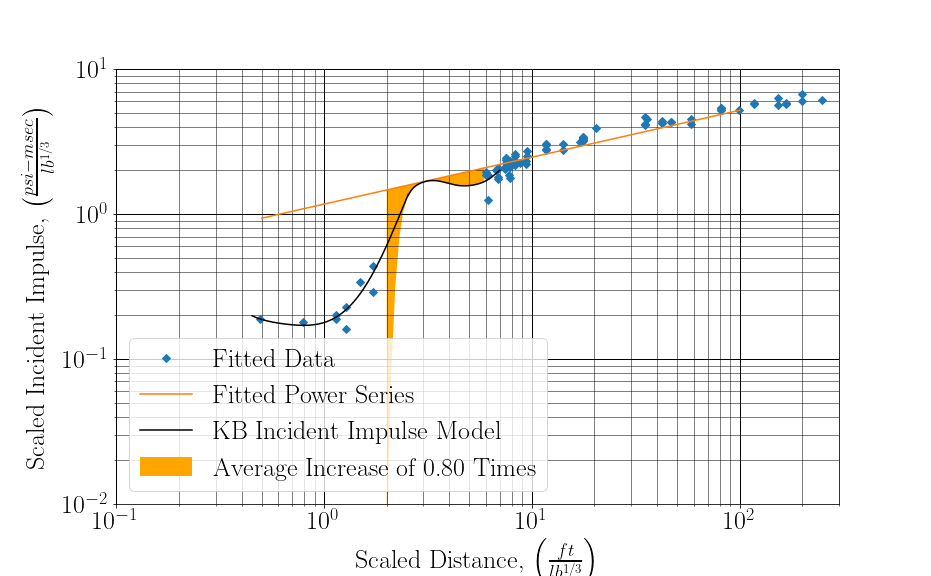
\includegraphics[width=6in]{/Users/skmcneill/Documents/Github/comprehensive/5_reports/figures/fig_ii_times_larger.png}
  \end{center}
  \caption{Average increase in the impulse due to the local maximum is approximately $15.36$ times the log linear fit of the KB incident impulse data that was less than or equal to a scaled distance of $2.5\:\frac{ft}{lb^{1/3}}$.}
\label{fig:KB_avg_inc}
\end{figure}%

\begin{figure}[tb]
  \begin{center}
   \includegraphics[width=6in]{/Users/skmcneill/Documents/Github/comprehensive/5_reports/figures/standoff_cost.png}
  \end{center}
  \caption{The effects of explosive standoff distance on the cost of various structural and non-structural components (adapted from \citep{Smith2016}).}
\label{fig:KB_cost}
\end{figure}%

It is hypothesized in this research, that the of afterburn of the products of reaction of TNT produce the local maximum observed in the KB incident impulse and positive phase duration.  The degree of afterburn is a function of the oxygen-balance of the explosive.  Therefore, other explosives with different oxygen-balances would produce different incident impulses at small scaled distances than predicted by the KB equations.
  
  
\begin{figure}[tb]
  \begin{center}
   \includegraphics[width=6in]{/Users/skmcneill/Documents/Github/comprehensive/5_reports/figures/ip_ppd_ii.png}
  \end{center}
  \caption{Kingery Bulmash postive phase duration plot showing the local maximum at a scaled distance of approximately $2.5\:\frac{ft}{lb^{1/3}}$\citep{Kingery1984}.}
\label{fig:KB_ppd}
\end{figure}%

\section{Statement of the Problem}
Detonations at small scaled-distances represent a common threat to the blast-resistant design of buildings, bridges and critical infrastructure due to proximity in urban areas and lack of protection in rural locations. The Kingery-Bulmash incident impulse curve used to predict the blasting loading shows significant non-linear behavior (local maximum) at small scaled distances.  This non-linear behavior at small scaled distances is not well understood.
In this research, the influence of explosive oxygen-balance on the non-linear behavior observed in the KB incident impulse curve will be examined. Three different explosives with increasing oxygen balance will be detonated and the following blast parameters will be measured:
\begin{itemize}
	\item incident-overpressure
	\item incident-impulse
	\item time-of-arrival
	\item positive-phase-duration
	\item fireball diameter
	\item fireball temperature.
\end{itemize}
Finally, a set of validation experiments will be conducted in a neutral atmosphere (no oxygen present) using the same explosives and measuring the same blast parameters. Our objective is to determine the degree to which differences in explosive oxygen-balance causes the non-linear behavior observed.  Additionally, a set of revised Kingery-Bulmash models will be developed that include the oxygen-balance as a parameter.

\section{Research and Scope Objectives}
The primary objective of this research is to quantify the effect explosive oxygen balance has on blast parameters at small scaled distances. This will lead to the secondary objective, the development of an improved Kingery Bulmash model that accounts for the oxygen balance of the explosive. The elements of these objectives include the following: 
\begin{itemize}
    \item determine the near field positive-phase-duration, incident impulse, and other relevant blast parameters of explosives with a range of oxygen balances,
    \item evaluate fireball diameter and temperature for explosives with a range of oxygen-balances.
    \item validate the influence of oxygen balance by detonating the same range of explosives in inert atmospheres, and
    \item develop a modified Kingery Bulmash model that accounts for oxygen balance.
\end{itemize}
 
\section{Originality of PhD Research}
This research is novel in hypothesizing a cause for the local maximum observed in the near field Kingery Bulmash incident impulse model. Currently, there is no clear and concise explanation for the observed effect. This research would aid in the design of blast resistant structures by providing more accurate models.
\section{Research Methodology}
This research will empirically determine the positive-phase-duration and incident-impulse of the following explosives:
\begin{itemize}
    \item trinitrotoluene (oxygen balance: -74\%),
    \item PETN (oxygen balance: -10\%)
    \item Dyno AP (oxygen balance: 0\%).
\end{itemize}
Pressure transducers will measure the time of arrival, incident impulse, and other blast parameters.  The explosives will be hemispherical in shape to minimize near-field shape effects.  The explosive charge will centered on a horizontal steel plate with incident pressure gauges positioned along a single axis.  Regression analysis will be used to describe the relationship between scaled distance, oxygen balance, and blast parameter data.

Simultaneous with the blast-parameter measurements, the fireball diameter and fireball temperature will be measured with a high-speed camera and spectrometer respectively.  Regression analysis will be used to determine a relationship between the oxygen balance and the fireball diameter and temperature.

A set of validation experiments will be conducted using the same explosives and incident pressure gauge configuration, but placed in an inert helium atmosphere.  If the hypothesis is correct, the oxygen balance of the explosives should not influence the positive phase duration or the incident impulse.

Finally, the Kingery Bulmash model will be modified to account for the explosive oxygen balance.  The new model will be a function of not just scaled distance but also the oxygen-balance of the explosive.
\section{Expected Contributions}
The expected contributions of this research are as follows:
\begin{itemize}
    \item development of improved Kingery-Bulmash models that account for the explosive oxygen-balance at small scaled distances,
    \item empirical evidence of blast parameters in the near field, and
    \item improved blast loading calculations for blast resistant designs.
\end{itemize}
\section{Academic Background Preparation of Candidate}
S. Kevin McNeill is currently a graduate student pursuing a Doctor of Philosophy in Explosive Engineering at Missouri University of Science and Technology (MST). He holds a Bachelors of Science in Mechanical Engineering from Louisiana State University and a Masters of Science in Explosive Engineering from MST. He is currently the Chief, of the Explosives Research and Development Division at the Bureau of Alcohol, Tobacco, Firearms, and Explosives (ATF).  In this position, he has conducted numerous government studies involving the measurement of overpressure and other blast parameters for the National Counter Terrorism Center, U.S. Army Corps of Engineers, Department of Defense Explosives Safety Board, and the Joint Improvised Explosive Device Agency.  In these studies, he has conducted test preparation, instrumentation selection, range layout, test controls, firing train selection, data analysis, and report writing.
%%
%% End of file `introduction.tex'.
